%Classe du document, A4, police taille 12
\documentclass[a4paper,12pt]{article}

% Dictionnaire français, pour caractères spéciaux, tirets, caractères accentués
\usepackage[french]{babel}
\usepackage[utf8]{inputenc}
%Toujours plus d'accents
\usepackage[T1]{fontenc}
\usepackage{lmodern}
\usepackage{indentfirst}
%Pour créer des paragraphes random
\usepackage{lipsum}  
%bibliographie
%Le style dépend du projet, voir avec le grand chef
%A mettre à l'endroit où vous voulez la faire apparaitre
%Donc dans le code pas ici t'as vu
%\bibliographystyle{ieeetr}
%\bibligraphy{nom_du_fichier.bib}

%hauteur entre deux lignes
\baselineskip 200cm
%hauteur entre deux paragraphes
\parskip 2mm
%longueur d'indentation
\parindent 2mm
%(on utilise \indent et \noindent sinon)

%Gérer ses marges

%Facilement
\usepackage[margin=2cm]{geometry}

%Commentaire sur plusieurs lignes
\usepackage{verbatim}

%Précisément
%\usepackage[left=2cm , right=2cm, bottom=2cm, top=2cm, headheight=2cm]{geometry} 
%header c'est l'en-tête pas la marge supérieure

%Toujours plus précisément
%\addtolength{\oddsidemargin}{-0.5in}
%\addtolength{\evensidemargin}{-5cm}
%\addtolength{\topmargin}{-0.5in}

%Faires des articles  plusieures colonnes
\usepackage{multicol}
%Separation des colonnes
\setlength{\columnsep}{2cm}

%Avoir des entêtes et pieds de page stylés
\usepackage{fancyhdr}
\pagestyle{fancy}
%Pour enlever l'entête avec les sections
%\fancyhf{}

%Ca se fait sous format \<pos><type>{<contenu>}
%type c'est "head" ou "foot"
%pos pour position gauche "l", droite "r" ou centre "c"
%contenu c'est ce que tu mets dans dedans 
%marche aussi avec des images mais flemme
%mettre un trait
%\renewcommand{\footrulewidth}{1.5pt}

% Liens dans le document
\usepackage{hyperref}  
% Légendes dans les environnements "figure" et "float"
\usepackage{subcaption}
%La base pour faire des figures juste
\usepackage{graphicx}
\usepackage[export]{adjustbox}
\usepackage{wrapfig}
%Trucs utiles pour les maths
\usepackage{amsmath}

\begin{document}
\begin{titlepage}
    \begin{center}
        \vspace*{0.5cm}
        
\includegraphics[scale=0.1]{logo_ponts.jpg}\\
        \vspace{0.7cm}
        {\Large ÉCOLE NATIONALE DES PONTS ET CHAUSSÉES}\\
        \vspace{4cm}
        \rule\linewidth{0.05cm}
        {\huge Recherche Opérationelle\par}
        \rule\linewidth{0.05cm}
        \vspace{1cm}
        {\Large Projet \par}
        \vspace{0.8cm}
        %{\Large }\\
        \vspace{0.3cm}
        {\large \textit{Nicolas BESSIN}}\\
        \vspace{0.3cm}
        {\large \textit{Erwann ESTEVE}}\\
        \vspace{0.3cm}
        {\large \textit{Tidiane POLO}}\\
        \vspace{1.2cm}
        
    \end{center}
\end{titlepage}

\section{Questions}
%\begin {enumerate}
%\item { 
    \textit{Q1 }
    Les contraintes suivantes sur $\mu$ permettent la linéarisation de $\mu = \alpha \beta$ avec $\alpha \in \lbrace 0,1 \rbrace$ et $\beta \in \lbrack 0, M \rbrack$ : 
    \begin{equation*}
        \begin{cases}
            \begin{alignedat}{2}
                &\mu \in [0,M] && \quad \text{(domaine de définition)}  \\ 
                &\mu \leq \alpha M && \quad  \text{(impose } \mu = 0 \text{ si }  \alpha = 0 \text{)}\\
                &\beta - (1 - \alpha)M \leq \mu \leq \beta && \quad \text{(impose } \mu = \beta \text{ si }  \alpha = 1 \text{)}
            \end{alignedat}
        \end{cases}
    \end{equation*}
%}
%\item {
    \textit{Q2 }
    Les contraintes suivantes sur $\mu$ et $\alpha$ permettent la linéarisation de $\mu = [\beta]^{+}$ avec $\beta \in \lbrack -M, M \rbrack$ : 
    \begin{equation*}
        \begin{cases}
            \begin{alignedat}{2}
                &\mu \in [0,M], \alpha \in \lbrace 0,1 \rbrace && \quad \text{(domaine de définition)} \\ 
                &\beta \leq M \alpha \leq M + \beta && \quad \text{(impose } \alpha = 1 \text{ si }  \beta > 0, \alpha = 0 \text{ si } \beta < 0 \text{)} \\
                &\beta - (1-\alpha)M \leq \mu \leq \beta + (1-\alpha)M && \quad \text{(impose } \mu = \beta \text{ si }  \alpha = 1 \text{)} \\
                &\mu \leq \alpha M && \quad \text{(impose } \mu = 0 \text{ si }  \alpha = 0 \text{)}
            \end{alignedat}
        \end{cases}
    \end{equation*}
    Notons que $\alpha$ est indéterminé pour $\beta = 0$, mais qu'on a tout de même $\mu = 0= [\beta]^{+}$.
%}
%\item {
    \textit{Q3 }
    Les contraintes suivantes sur $\gamma$ et $\delta$ permettent la linéarisation de $ \gamma = min(\alpha, \beta)$ avec $\alpha, \beta \in \lbrack -M, M \rbrack$ : 
    \begin{equation*}
        \begin{cases}
            \begin{alignedat}{2}
                &\gamma \in [-M,M], \delta \in \lbrace 0,1 \rbrace && \quad \text{(domaine de définition)} \\ 
                &2M(\delta - 1) \leq \beta - \alpha \leq 2M \delta && \quad \text{(impose } \delta = 1 \text{ si }  \beta > \alpha \text{, }\delta = 0 \text{ si }  \beta < \alpha \text{)}\\
                &\beta - 2M\delta \leq \mu \leq \beta + 2M\delta && \quad \text{(impose } \gamma = \beta \text{ si }  \beta < \alpha \text{)}\\
                &\alpha - 2M(1-\delta) \leq \mu \leq \alpha + 2M(1-\delta) && \quad \text{(impose } \gamma = \alpha \text{ si }  \beta > \alpha \text{)}
            \end{alignedat}
        \end{cases}
    \end{equation*}
    Noton que $\delta$ est indéterminé pour $\alpha = \beta$, mais qu'on a tout de même $\gamma = \alpha = \beta = min(\alpha, \beta)$.
    
    \underline{Autre méthode} \\
    On introduit les variables binaires $y_\alpha$ et $y_\beta$, et la variable continue $y$.
    Le problème s'écrit alors :
    \begin{equation}
        \begin{alignedat}{2}
            \min _{\alpha, \beta, y_\alpha, y_\beta, y} & y \\
            \text{ s.c. } 
            &y \geq \alpha - 2M y_\alpha, & \quad& y \geq \beta - 2M y_\beta \\
            &y_\alpha + y_\beta = 1 \\
        \end{alignedat}
    \end{equation}
    La contrainte $y_\alpha + y_\beta = 1$ assure  $y = \alpha$ ou $y = \beta$.
    De plus, puisque c'est un problème de minimisation, on a bien $y = min(\alpha, \beta)$. \\
    %\textit{N.B. : Nous avons trouvé cette élégante méthode à \underline{\href{https://doi.org/10.3390/math10020283}{ce lien}}.}
%}
%\item {
    \textit{Q4 }
    \begin{comment}
        On a le problème suivant : 
        \begin{equation}
            \begin{aligned}
                \min _{\alpha, \beta, \gamma} & \max (\alpha, \beta) + \gamma \\
                \text{ s.c. } & A(\alpha, \beta, \gamma)^T \leq b \\
            \end{aligned}
        \end{equation}
    \end{comment}
    On introduit la variable continue $\delta$ et les contraintes suivantes :
    $$ \delta \geq \alpha, \qquad \delta \geq \beta $$
    Le problème initial s'écrit alors :
    \begin{equation}
        \begin{aligned}
            \min _{\alpha, \beta, \gamma, \delta}  \delta &+ \gamma \\
            \text{ s.c. }  A(\alpha, \beta, \gamma)^T &\leq b \\
            \alpha &\leq \delta \\
            \beta &\leq \delta \\
        \end{aligned}
    \end{equation}
%}
%\item{
    \textit{Q5 }
    Considérons le problème suivant :
    \begin{equation}
        \begin{aligned}
            \min _{a, b, c} & \lbrack a - \min(b, c) \rbrack^+ \\
        \end{aligned}
        \label{linmin}
    \end{equation}

    On a $ \forall b, c : -\min(b, c) = \max(-b, -c) $ \\
    Puisque c'est un problème de minimisation, on peut écrire :
    \begin{equation}
        \eqref{linmin} \iff
        \begin{aligned}
            \min _{a, b, c, d} & d \\
            \text{ s.c. } & d \geq 0 \\
            & d \geq a - \min(b, c) \\
        \end{aligned}
        \iff
        \begin{aligned}
            \min _{a, b, c, d, e} d \\
            \text{ s.c. }
            d &\geq 0 & \quad& d \geq a + e \\
            e &\geq -b & \quad& e \geq -c \\   
        \end{aligned}
    \end{equation}
    

    Pour linéariser les termes $p_f(v, x, y) c^c(C^f(v, x, y, z ,\omega))$, on doit distribuer la multiplication
    (On sait linéariser les multiplications de variables binaires et de variables continues). On a donc :
    $$ p_f(v, x, y) c^c(C^f(v, x, y, z ,\omega)) = (\sum _ {s \in S} p_s x_{vs} + \sum _{q \in Q_0} p_q y _{eq}) (c^c(C^f(v, x, y, z ,\omega)))  $$
    où $c^c(C^f(v, x, y, z ,\omega))$ est une variable continue, issue du regroupement des composantes du coût et de la linéarisation de la pénalité.
    $$
    \begin{aligned}
        p_f(v, x, y) c^c(C^f(v, x, y, z ,\omega)) &= \sum _ {s \in S} p_s x_{vs} (c^c(C^f(v, x, y, z ,\omega))) \\
        &+ \sum _{q \in Q_0} p_q y _{eq} (c^c(C^f(v, x, y, z ,\omega)))
    \end{aligned}
    $$

    On a donc besoin d'une borne supérieure pour $C^f(v, x, y, z ,\omega)$

    Même raisonnement pour $(1 - \sum _{v \in V^s} p_f(v)) c^c(C^n(\omega))$ :

    $$ \lbrack 1 - \sum _{v \in V^s} p_f(v) \rbrack c^c(C^n(\omega)) = 
    c^c(C^n(\omega)) - \sum _{v \in V^s} \lbrack \sum _{s \in S} p_s x_{vs} c^c(C^n(\omega)) + \sum _{q \in Q_0} p_q y _{eq} c^c(C^n(\omega)) \rbrack  $$

    La PLNE peut alors s'écrire (notons $e = (v_{0},v)$, $N^{turbine} =$ nombre de turbine) :
    \begin{align*}
        & \min_{x,y,z} C_{c}+C_{o} \\
        & \text{s.c. \text{ (1), (2), (3), (4)  (conditions du sujet)}} 
    \end{align*}
    \begin{equation}
        \begin{cases}
            \begin{alignedat}{3}
                & (x_{v,s}) \in \{0,1\}^{V^{s} \times S}, && (y_{e,q}^{land}) \in \{0,1\}^{V^{s} \times Q}, (z_{v,t})\in \{0,1\}^{V^{s} \times V^{t}}&&, (y_{u,v,q}^{sub}) \in \{0,1\}^{V^{s} \times V^{s} \times Q}\\
                & \sum_{q \in Q_0} y_{u,v,q}^{sub} = 0, && y_{u,v,q}^{sub} =  y_{v,u,q}^{sub}  && \text{for } u \in V^s, v \in V^s, q \in Q_0 \\
            \end{alignedat}
        \end{cases}
    \end{equation}
    \begin{equation}
        \begin{cases}
            \begin{alignedat}{2}
                & (N_v^{linkTurbine}) \in R^{V^s}, (Capa_v^{linMin}) \in R^{V^s}, (Curt_{v,\omega}) \in R^{V^s \times \Omega},(Curt_\omega^{noFail}) \in R^{\Omega},&& (Curt_{v, \omega}^{ownFail}) \in R^{V^s \times \Omega} \\
                & N_v^{linkTurbine} = \sum_{t \in V^t} z_{v,t} && \text{for } v \in V^s \\
                & Capa_v^{linMin} \geq - \sum_{s \in S} r_s * x_{v,s}, \quad Capa_v^{linMin} \geq - \sum_{q \in Q_0} r_q * y_{e,q}^{land}  &&  \text{for } v \in V^s  \\
                & Curt_{v,\omega} \geq 0, Curt_{v,\omega} \geq \pi_\omega * N_v^{linkTurbine} + Capa_v^{linMin}  &&  \text{for } v \in V^s, \omega \in \Omega  \\
                & Curt_\omega^{noFail} = \sum_{v \in V^s} Curt_{v,\omega} && \text{for } \omega \in \Omega \\
                & Curt_{v, \omega}^{ownFail} \geq 0, \quad Curt_{v, \omega}^{ownFail} \geq \pi_\omega * N_v^{linkTurbine} - \sum_{u \in V^s, q \in Q_0} r_q * y_{v,u,q}^{sub}  &&  \text{for } v \in V^s, \omega \in \Omega \\
            \end{alignedat}
        \end{cases}
    \end{equation}
    \begin{equation}
        \begin{cases}
            \begin{alignedat}{2}
                & (Curt_{v, \omega}^{ownFail}) \in R^{V^s \times \Omega} \\
                & Curt_{v, \omega}^{ownFail} \geq 0, \quad Curt_{v, \omega}^{ownFail} \geq \pi_\omega * N_v^{linkTurbine} - \sum_{u \in V^s, q \in Q_0} r_q * y_{v,u,q}^{sub} \quad &&  \text{for } v \in V^s, \omega \in \Omega \\
            \end{alignedat}
        \end{cases}
    \end{equation}
    \begin{equation}
        \begin{cases}
            \begin{alignedat}{2}
                & (P_{u,v,\omega}^{sendOtherFail}) \in R^{{V^s}^2 \times \Omega}, 1_{u,v,\omega}^{powerSend} \in \{0,1\}^{{V^{s}}^2 \times \Omega},  1_{u,v,\omega}^{cableCapa} \in && \{0,1\}^{{V^{s}}^2 \times \Omega} \\
                & 1_{u,v,\omega}^{powerSend} + 1_{u,v,\omega}^{cableCapa} = 1 && \text{for } (u,v) \in {V^s}^2, \omega \in \Omega \\
                & P_{u,v,\omega}^{sendOtherFail} \geq N_v^{linkTurbine} * \pi_\omega - 1_{u,v,\omega}^{cableCapa} * P^{max} * N^{turbine}
            \end{alignedat}
        \end{cases}
    \end{equation}
    \begin{equation}
        \begin{cases}
            \begin{alignedat}{2}
                & (Curt_{u,v,\omega}^{otherFail}) \in R^{{V^s}^2 \times \Omega}, (Curt_{v,\omega}^{fail}) \in R^{V^s \times \Omega} \\
                & Curt_{u,v,\omega}^{otherFail} \geq 0 && \text{for } (u,v) \in {V^s}^2, \omega \in \Omega \\
                & Curt_{u,v,\omega}^{otherFail} \geq p_\omega * N^{turbine} + P_{u,v,\omega}^{sendOtherFail} + Capa_v^{linMin} \quad && \text{for } (u,v) \in {V^s}^2, \omega \in \Omega \\
                & Curt_{v,\omega}^{fail} = curt_{v,\omega}^{ownFail} + \sum_{u \in V^s} Curt_{v,u,\omega}^{otherFail} \quad && \text{for } v \in V^s, \omega \in \Omega \\
            \end{alignedat}
        \end{cases}
    \end{equation}
    \begin{equation}
        \begin{cases}
            \begin{alignedat} {2}
                & (C_{v}^{substation}) \in R^{V^{s}}, (C_{v}^{landcable}) \in R^{V^{s}}, (C_{u,v}^{subcable}) \in R^{{V^{s}}^{2}}, C_{v,t}^{turbine} \in R^{V^{s} \times V^{t}}, && C^{c} \in R \\
                & C_{v}^{substation} = \sum_{s \in S} c_{s} * x_{v, s}, \quad C_{v}^{landcable} = \sum_{q \in Q_0} y_{v,q}^{land}*(c_{q}^{f} + c_{q}^{l} l_{e}) && \text{for }  v \in V^{s} \\
                & C_{u,v}^{subcable} = \sum_{q \in Q_0} y_{u,v,q}^{sub} * (c_{q}^{f}+c_{q}^{l} l_{(u,v)}),\quad C_{v}^{turbine} = \sum_{q \in Q_0} z_{v,t}*(c_{t}^{f} + c_{t}^{l} l_{(v,t)}) && \text{for }  (u,v) \in {V^{s}}^{2}, t \in V^{t} \\
                & C^{c} = \sum_{v \in V^s} C_{v}^{substation} + \sum_{v} C_{v}^{landcable} + \sum_{u \in V_{s},v \in V_{s}} C_{u,v}^{subcable} + \sum_{v \in V^s, t \in V^{t}} C_{v,t}^{turbine} \\
            \end{alignedat}
        \end{cases}
    \end{equation}
    \begin{equation}
        \begin{cases}
            \begin{alignedat}{2}
                & (C_{v,\omega}^{curtNoFail}) \in R^{V_{s} \times \Omega}, (C_{v,\omega}^{curtFail}) \in R^{V^{s} \times \Omega} \\
                & C_{v,\omega}^{curtNoFail} \geq c^{0}Curt_{v,\omega}^{noFail}, C_{v,\omega}^{curtNoFail} \geq c^{0}Curt_{v,\omega}^{noFail} + c^{p}(Curt^{noFail}-C^{max}) \quad &&  \text{for } \omega \in\Omega, v \in V^{s} \\
                & C_{v,\omega}^{curtFail} \geq c^{0}Curt_{v,\omega}^{fail}, \quad C_{v,\omega}^{curtFail} \geq c^{0}Curt_{v,\omega}^{fail} + c^{p}(Curt^{fail}-C^{max}) \quad && \text{for } \omega \in\Omega, v \in V^{s} \\
            \end{alignedat}
        \end{cases}
    \end{equation}
    \begin{equation}
        \begin{cases}
            \begin{alignedat}{2}
                & (C_{v,\omega}^{wCurtFail}) \in R^{V^{s} \times \Omega}, (x_{v,s,\omega}^{timeCurtCostFail}) \in R^{V^{s} \times S \times \Omega},(y_{e,q, \omega}^{timeCurtCostFail}) \in && R^{V^{s} \times Q \times \Omega} \\
                & x_{v,s,\omega}^{timeCurtCostFail} \leq x_{v,s} * C_{max}, \quad x_{v,s,\omega}^{timeCurtCostFail} \leq C^{curtFail} && \text{for } \omega \in\Omega, v \in V^{s}, s \in S\\
                & x_{v,s,\omega}^{timeCurtCostFail} \geq C^{curtFail} - (1 - x_{v,s})*C_{max}, \quad x_{v,s,\omega}^{timeCurtCostFail} \geq 0 && \text{for } \omega \in\Omega, v \in V^{s}, s \in S\\
                & y_{e,q,\omega}^{timeCurtCostFail} \leq y_{v,q}^{land}*C_{max}, \quad y_{e,q,\omega}^{timeCurtCostFail} \leq C_{v,\omega}^{curtfail} && \text{for } \omega \in\Omega, v \in V^{s}, q \in Q\\
                & y_{e,q,\omega}^{timeCurtCostFail} \geq C_{v,\omega}^{curtfail} - (1 - x_{v,s})*C_{max}, \quad y_{e,q,\omega}^{timeCurtCostFail} \geq 0  && \text{for } \omega \in\Omega, v \in V^{s}, q \in Q\\
                & C_{v,\omega}^{wCurtFail} = \sum_{s \in S} x_{v,s, \omega}^{timeCurtCostFail}*p_{s} + \sum_{q \in Q} y_{e,q,\omega}^{timeCurtCostFail} * p_{q} && \text{for } \omega \in\Omega, v \in V^{s}\\
            \end{alignedat}
        \end{cases}
    \end{equation}
    \begin{equation}
        \begin{cases}
            \begin{alignedat}{2}
                & (x_{v,s,\omega}) \in R^{V^{s} \times Q_{0}, \Omega}, (y_{e,q,\omega}) \in R^{V^{s} \times Q_{0}, \Omega} \\
                & x_{v,s,\omega}^{TimeCurt} \leq x_{v,s}*C_{max}, \quad x_{v,s,\omega}^{TimeCurt} \leq C_{\omega}^{fail} &&\quad \text{for } \omega \in\Omega, v \in V_{s}, s \in S\\
                & x_{v,s,\omega}^{TimeCurt} \geq C_{\omega}^{fail}-(1-x_{v,s})*C_{max}, \quad x_{v,s,\omega}^{TimeCurt} \geq 0 &&\quad \text{for } \omega \in\Omega, v \in V_{s}, s \in S\\
                & y_{e,q,\omega}^{TimeCurt} \leq y_{v,q}^{land} * C_{max}, \quad y_{e,q,\omega}^{TimeCurt} \leq C_{\omega}^{fail} \quad && \text{for } \omega \in \Omega, q \in Q_{0}, v \in V^{s} \\
                & y_{e,q,\omega}^{TimeCurt} \geq C_{\omega}^{fail}-(1-y_{v,q}^{land})*C_{max}, \quad  y_{e,q,\omega}^{TimeCurt} \geq 0 \quad && \text{for } \omega \in\Omega, q \in Q_{0}, v \in V^{s}\\
            \end{alignedat}
        \end{cases}
    \end{equation}
    \begin{equation}
        \begin{cases}
            \begin{alignedat}{2}
                & (C_{\omega}^{fail}) \in R^{\Omega}, (C_{\omega}^{nofail}) \in R^{\Omega}, C_{o} \in R\\
                & (C_{\omega}^{fail}) = \sum_{v \in V_{0}} C_{v,\omega}^{wCurtFail} &&\quad \text{for } \omega \in \Omega \\
                & C_{\omega}^{nofail} = C_\omega^{curtailement} - \sum_{v \in V_{s},s \in S} x_{v,s,\omega}^{TimeCurt}*p_s - \sum_{v \in V^s, q \in Q_{0}} y_{e,q,w}^{TimeCurt}*p_{q} && \quad \text{for } \omega \in \Omega \\
                & C_{o} = \sum_{\omega \in \Omega} p_{\omega} * (C_{\omega}^{fail} + C_{\omega}^{nofail}) \\
            \end{alignedat}
        \end{cases}
    \end{equation}

    \textit{N.B. : la justification de cette formulation du PLNE est trouvable étape par étape dans les commentaires du document linearSolverCode.jl}
%}


%\end{enumerate}

\section {Algorithm}
Une fois le solveur linéaire mis en place, le problème principal qui empêche de l'utiliser pour les instances medium, large et huge est la taille de celles-ci - en effet, le nombre de variable dans le modèle influe énormément sur le temps de calcul (et donc la possibilité de résoudre le problème). 
Ainsi nous avons implémenté la stratégie suivante :
\begin{itemize}
    \item Réduire la taille de l'instance avec différente méthode (voir ci-dessous) .
    \item Résoudre le problème pour cette sous-instance avec le solveur linéaire
    \item Transformer la solution obtenue en une solution du problème initial.
\end{itemize}
Les stratégies de réduction de taille que nous avons implémenté sont motivées par les observations suivantes que nous avons pu faire sur l'instance small :
Seuls certains sites de sous-station sont utilisés (voir figure 1), et seuls certains types de sous-station et de câbles sont utilisés (voir figure 2).

\begin{figure}[h]
    \centering
    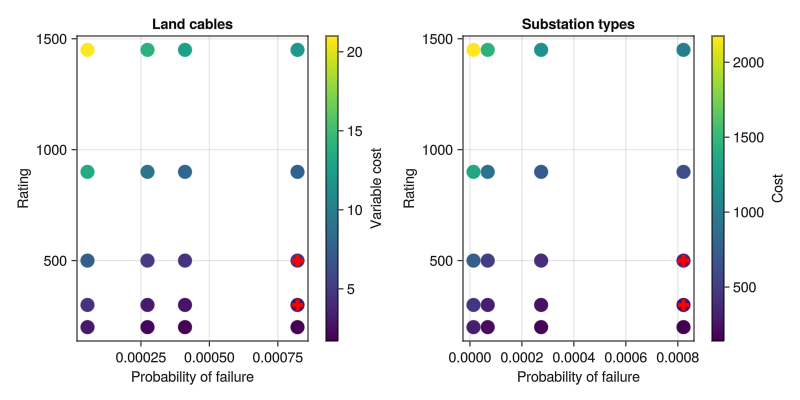
\includegraphics[scale=0.5]{small-types.png}
    \caption{Types des sous-stations et des câbles dans l'instance small - en rouge, les types effectivement utilisés dans la solution optimale}
\end{figure}

\begin{itemize}
    \item Ne garder que les sites de sous-station les plus proches des éoliennes (comme avec la solution optimale de l'instance small)
    \item Remplacer les multiples scénarios par un unique scénario représentatif (e.g. un scénario dont la puissance est $p = p_{min} + x(p_{max} - p_{min})$ avec $x$ un coefficient choisi, e.g $x = 0.95$)
    \item Éliminer certains types possibles de sous-stations et / ou de câbles, en fonction de leurs probabilités de panne et de leurs coûts.
\end{itemize}

L'intérêt de ces stratégies est le suivant : si on note $n_{SubSites}$ le nombre de sites de sous-station, $n_{SubTypes}$ le nombre de types de sous-station, $n_{LandCables}$ le nombre de types de câbles liant à la terre, $n_{SubCables}$ le nombre de types de câble reliant des sous-stations, $n_{Scenarios}$ le nombre de scénarios, et $n_{t}$ le nombre d'éoliennes, alors le nombre de variables du problème - et donc le temps de calcul - est de l'ordre de 
$$ O(n_{SubSites} \times n_{SubTypes} + n_{LandCables} \times n_{SubSites} + n_{SubSites}^2 \times n_{SubCables} + n_{Scenarios} \times n_{t} \times n_{SubSites} \times n_{SubTypes}) $$

Avec ces stratégies, nous pouvons utiliser le solveur linéaire pour résoudre les instances. Les meilleurs scores obtenus sont les suivants :

\begin{table}[h]
    \centering

    \begin{tabular}{lllll}
    size & small         & medium       & large   & huge    \\ \hline
    cost & 3244          & 6472         & 8566    & 5583    \\
    gap  & $\leq 3.8 \%$ & $\leq 7.5\%$ & Unknown & Unknown \\ \hline
    \end{tabular}

\end{table}

Le gap est calculé par rapport à la solution du relaché linéaire, et est donc une sur-estimation du gap par rapport à la solution optimale entière.
(Pour large \& huge, nous n'avons pas pu calculer le gap, 16Go de RAM n'étant pas suffisant pour les résoudre.)


\end{document}


